	\newpage
\section{Projektowanie}		%3
%Napisać z jakich narzędzi będziemy korzystać (kompilator, język programowania), git, biblioteki dodatkowe, itp.
%Opisać szczegółowe ustawienia kompilatora (jeśli są), powiązania z bibliotekami, itp.
%Narysować graf, UML, diagram klas, schemat działania algorytmu
%Jeśli zadanie zakłada przedstawienie jakiegoś narzędzia (np. git, AI) należy opisać sposób jego używania

\subsection{Implementacja Algorytmu}

Do zaimplementowania Algorytmu obliczania $\pi$ zostanie użyty Język \texttt{C++} z kompilatorem \texttt{g++}. Wersja standardu \texttt{C++} to \texttt{C++23}. Systemem budowy projektu będzie \texttt{CMake}, pomagający w konfiguracji wersji kompilatora czy bibliotek. \texttt{CMake} pozwala na generowanie plików budujących dany projekt, zgodnie z określoną konfiguracją. Oszczędza to programiście, szczególnie przy większych projektach, manualne pisanie Makefileów.
Plik konfiguracyjny \texttt{CMakeLists.txt} może wyglądać jak na rysunku

\begin{lstlisting}[caption=Plik konfiguracyjny CMake, label={lst:cmakelists}, language=C++]
	cmake_minimum_required(VERSION 3.15)
	
	set(PROJECT_NAME proj4)
	
	project(${PROJECT_NAME} VERSION 0.1 LANGUAGES CXX)
	
	set(CMAKE_CXX_STANDARD 23)
	set(CMAKE_CXX_STANDARD_REQUIRED ON)
	set(CMAKE_EXPORT_COMPILE_COMMANDS True)
	set(CMAKE_RUNTIME_OUTPUT_DIRECTORY ${CMAKE_CURRENT_LIST_DIR}/out)
	
	add_subdirectory(src)
	
\end{lstlisting}

Edytorem będzie program Neovim. Jest to terminalowy edytor tekstu z możliwością poszerzenia funkcjonalności przy użyciu wszelkiego rodzaju pluginów. Wybrany został, dlatego że jest on już skonfigurowany na moim komputerze zgodnie z moimi preferencjami.

\subsection{Git}

Dla ułatwienia pracy, zastosowany został front-end dla gita o nazwie lazygit. Jest to terminalowy program, którego główną zaletą jest łatwa nawigacja przy użyciu klawiatury. Ponadto, jest on lekki i szybki.

\subsection{Doxygen}

Konfiguracja dla Doxygena jest wygenerowana przy użyciu programu doxywizard, pokazany na rys. \ref{fig:doxywizard}, pozwalającego na graficzne zmienianie ustawień. Po wygenerowaniu konfiguracji, Doxygen wywoływany jest przy użyciu komendy.

\begin{figure}[H]
	\centering
	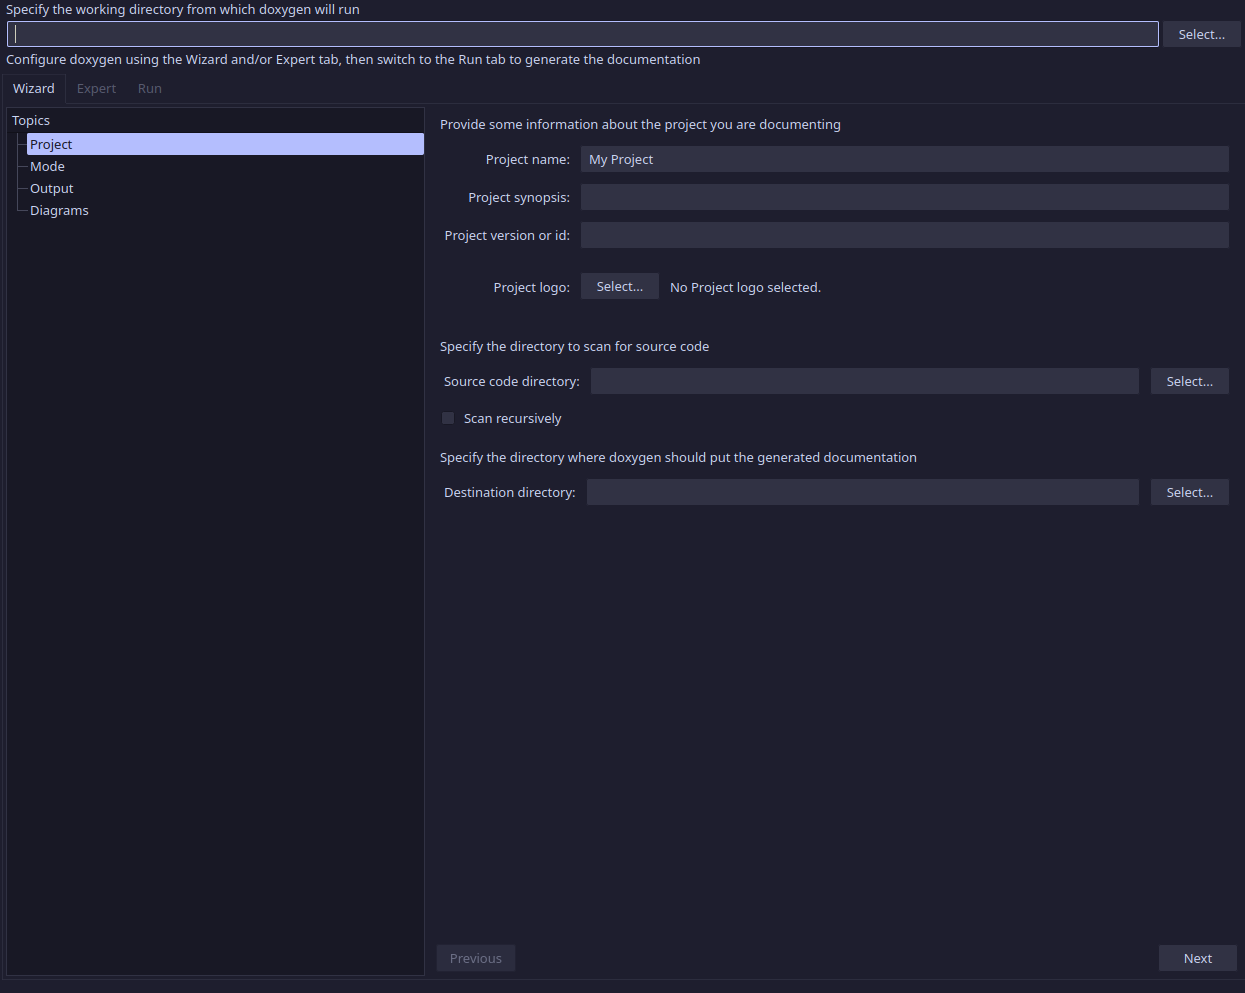
\includegraphics[width=1\textwidth]{images/doxywizard.png}
	\caption{\centering{Interfejs programu doxywizard}}
	\label{fig:doxywizard}
\end{figure}

\subsection{Github Copilot}
Do napisania programu do pomocy został wykorzystany Github Copilot. Z pomocy Copilota można skorzystać na 3 sposoby. Sposób pierwszy - poprzez podpowiedzi generowane przez Copilota które są oznaczone kolorem szarym, co pokazano na rysunku nr \ref{fig:copilotsuggestion}.

\begin{figure}[H]
	\centering
	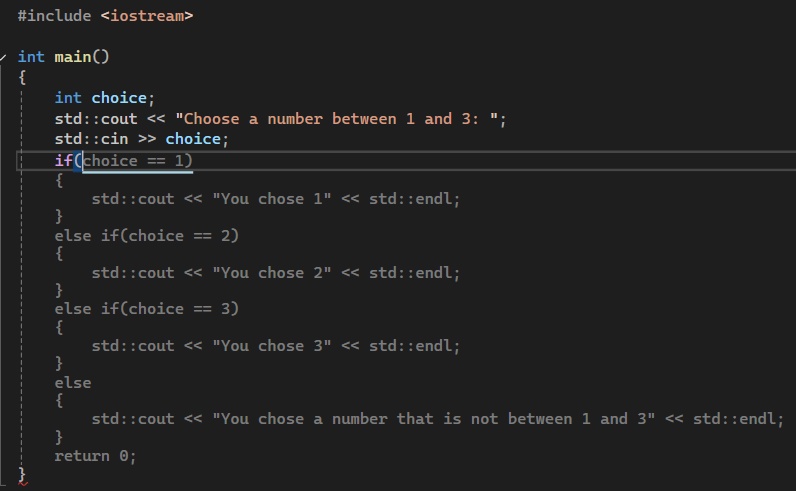
\includegraphics[width=1\linewidth]{images/CopilotSuggestion}
	\caption{\centering{Sugerowanie przez copilot}}
	\label{fig:copilotsuggestion}
\end{figure}

Sposób drugi to standardowe okienko chat gdzie można zapytać go o rzeczy związane z kodem, przedstawione zostało na rysunku nr \ref{fig:copilotchat}

\begin{figure}[H]
	\centering
	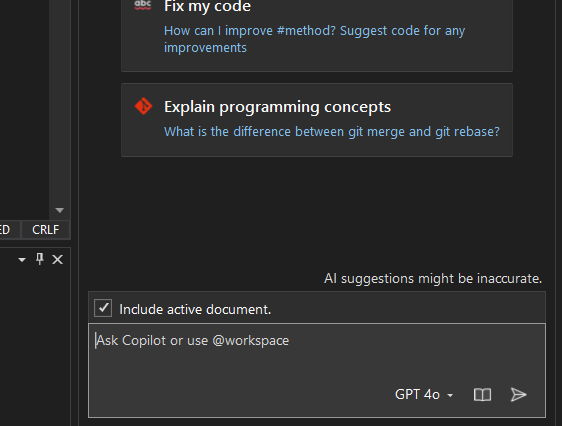
\includegraphics[width=1\linewidth]{images/CopilotChat}
	\caption{\centering{okienko chat Copilot}}
	\label{fig:copilotchat}
\end{figure}

Trzeci sposób to wykorzystanie komentarzy jako poleceń co ma zrobić copilot, jak pokazano na rysunku nr \ref{fig:copilotcomments}

\begin{figure}[H]
	\centering
	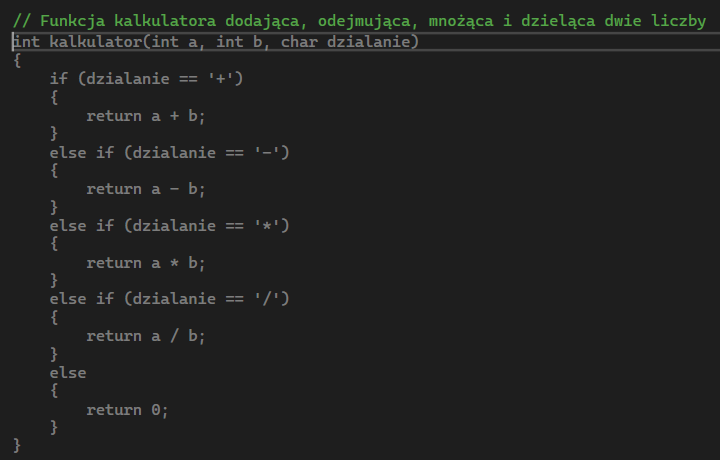
\includegraphics[width=1\linewidth]{images/CopilotComments}
	\caption{\centering{Zastosowanie komentarzy do generowania kodu}}
	\label{fig:copilotcomments}
\end{figure}
